\section{Physics of Nuclear Energy}
\label{sec:Physics of Nuclear Energy}

	The energy released from any reaction is dictated by Einstein's famous equation: \cite{bibid}
	%
	\begin{equation}
		E = mc^2
	\end{equation}
	%
	where $E$ is the so called rest mass energy of an object with mass $m$ and $c$ is the speed of light. To calculate the energy release of a reaction, one simply subtracts the rest mass energy of the initial state from the final state such that:
	%
	\begin{equation}
		\Delta E \equiv Q = \left(\sum m_i - \sum m_f \right) c^2
		\label{eq:reactionEnergyRelease}
	\end{equation}
	%
	Here $m_i$ is the masses of any initial components (particles in our context) and $m_f$ is the masses of any final components. It is a common misconception that equation \ref{eq:reactionEnergyRelease} only applies to nuclear reactions, but in reality chemical reactions are described by the same physics. Some example reactions are shown in Table \ref{tab:reactionEnergyReleases}. 
	
	\begin{table}[!h]		
		\caption{Mass differences and energy released by various reactions}
		\centering
		\tabulinesep = 1.5mm		
		\begin{tabu}{|c|c|c|c|}
			\hline
			Reaction & Type & $\left(\sum m_i - \sum m_f \right)$ & $Q$ \\
			\hline
			p + e$^-$ $\rightarrow$ $^1$H & Recombination & $1.46\times10^{-8}$ amu & 13.6 eV\\
			n + $^{235}$U $\rightarrow$ $^{140}$Xe + $^{94}$Sr + 2n & Fission & 0.198 amu & 184.7 MeV\\
			$^{2}$H + $^{3}$H $\rightarrow$ $^{4}$He + n & Fusion & 0.0189 amu & 17.6 MeV \\ 
			\hline
		\end{tabu}
		\label{tab:reactionEnergyReleases}
	\end{table}

	For us to produce energy, we ultimately seek to find reactions that produce large $Q$. To do this we need reactants with large $m_i$ relative to the $m_f$ of the products. To aid in determining this, the masses of several isotopes are shown plotted in Figure \ref{fig:massPerNuclide}.
	
	
	\begin{figure}
		\centering
		\includegraphics[scale=0.7]{massPerNuclide}
		\caption{Mass per nuclide of various isotopes. All exothermic fusion reactions must occur between isotopes lighter than $^{56}$Fe and all exothermic fission reactions must occur between isotopes heavier than $^{56}$Fe. }
		\label{fig:massPerNuclide}
	\end{figure}

	As we can see, the isotope with the smallest mass per nuclide is $^{56}$Fe. It is considered the most efficiently bound nuclide since it's corresponding rest mass energy per nuclide is lower than any other isotope. This means that for any isotopes lighter than ${^{56}}$Fe, we can gain energy by combining them (fusion) into heavier isotopes. Similarly, we gain energy by breaking up isotopes (fission) with mass greater than $^{56}$Fe. It is interesting to note the local minimum mass per nuclide of $^4$He. Due to it's unique position, fusion reactions that produce it will be particularly energetic. Interestingly, it also means that the fission of $^6$Li is uniquely exothermic. The exact reason for why isotope masses behave in this way is a topic of nuclear physics beyond the scope of this discussion. 
	
	Moving forward, we will adopt short-hand notations for a few light isotopes of particular interest to fusion. These isotopes are listed in Table \ref{tab:isotopeShorthands}.
	
	\begin{table}[h!]
		\centering
		\tabulinesep = 1.5mm
		\caption{Short hand notations for a few light isotopes of particular interest to nuclear fusion}
		\begin{tabu}{|c|c|c|}
			\hline
			Name & Proper Notation & Short Hand \\\hline
			Deuteron & $^2$H & D \\
			Triton & $^3$T & T \\
			Alpha Particle & $^4$He & $\alpha$ \\
			\hline 
		\end{tabu}
		\label{tab:isotopeShorthands}
	\end{table}
	
	With this notation in mind, there are a few fusion reactions that are of particular interest for energy production. 
	
	\begin{eqnarray}
			\text{D + D} &\rightarrow& \text{T + p + 4.03 MeV}  \label{eq:DDp}\\
			\text{D + D} &\rightarrow& ^3\text{He + n + 3.27 MeV} \label{eq:DDn}\\
			\text{D + T} &\rightarrow& \alpha \text{ + n + 17.6 MeV} \label{eq:DTn}\\
			\text{D + } ^3\text{He} &\rightarrow& \alpha \text{ + p + 18.3 MeV} \label{eq:D3Hep} \\
			\text{p + } ^{11}\text{B} &\rightarrow& 3\alpha	\text{ + 8.7 MeV} \label{eq:p11B}		
	\end{eqnarray}

	These reactions are primarily chosen due to the availability of the reactants, the amount of energy released, and the ease to which they can be made to fuse. The last of these criteria is described by the reaction's fusion cross-section ($\sigma$). Cross sections are essentially the probability (normalized for density and path length) that two particles will interact, or in our case fuse. As such, the cross section determines the reaction rate between two species. Formally the volumetric reaction rate between species 1 and 2 is given by:  
	%
	\begin{equation}
		\mathcal{R}_{12} = \int dv_1^3 \int dv_2^3 f_1(\vec{v}_1) f_2(\vec{v}_2) \sigma_{12} \left|\vec{v}_1 - \vec{v}_2\right|
		\label{eq:reactionRate}
	\end{equation}
	%
	where $f_1$ and $f_2$ are the velocity distribution functions of species 1 and 2 respectively and $\vec{v}_1$ and $\vec{v}_2$ are the velocities of species 1 and 2 respectively. The cross sections for all of the listed reactions are shown in Figure \ref{fig:crossSections}. 
	
	\begin{figure}[h!]
		\centering
		\includegraphics[scale=0.7]{crossSections}
		\caption[Fusion Cross-Sections]{Cross sections of various fusion reactions consider for fusion energy. The cross sections for equations \ref{eq:DDp} - \ref{eq:p11B} are shown as green, green, red, blue, and yellow curves respectively. The cross sections for equations \ref{eq:DDp} and \ref{eq:DDn} are nearly identical up until very high energies. Equation \ref{eq:DDp} is dashed and equation \ref{eq:DDn} is solid. Cross sections here are plotted as a function of their center of mass energies. }
		\label{fig:crossSections}
	\end{figure}

	As we can see there are many orders of magnitude separating the cross-sections of these reactions depending on the center of mass energy. DT fusion (equation \ref{eq:DTn}), is by far the easiest to achieve having a max cross section of about 5 barns. For context this is roughly 100 times less than the thermal fission cross section of $^{235}$U. Following DT, DD fusion (equations \ref{eq:DDp} and \ref{eq:DDn}) is the next easiest to achieve at reasonable energies. For this reason, most major fusion experiments in the world aim for DT fusion as this will be the reaction that powers the first generation of nuclear fusion reactors. The other reactions listed have their advantages such as higher fuel availability or being aneutronic (emitting no neutrons) but will be reserved for second or third generation fusion reactors.
	
	An important thing to note about these cross sections is the rather high center of mass energies required to achieve them. For reference, the fission cross section quoted previously occurs at room temperature energies (0.0253 eV) whereas the maximum DT cross section occurs at about 65 keV. This corresponds to temperatures of 750 million degrees Celsius (1.3 billion degrees Fahrenheit). This is because all fusion reactions require combining nuclides that are both positively charged leading to a Coulomb repulsion that can only be overcome with extreme energies. This Coulomb repulsion is also why the fusion of hydrogen atoms (who have the lowest possible charge) requires less energy than the reactions involving helium or boron. This is the primary challenge of nuclear fusion; creating and maintaining these extreme conditions. 
	
	Perhaps the most naive way to achieve nuclear fusion is through the acceleration of particles into a solid target. In fact this works remarkably well and is still the source of many fusion experiments to date. However, this approach to fusion is inefficient and cannot be used to generate net power. This is because the accelerated particle loses energy to Coulomb collisions with the solid target at a rate much higher than the fusion rate. A 100 keV triton, for example, travels less than 1 um into a solid target of pure deuterium before loosing all of its energy. This is compared to the 6000 um "mean fusion path length" one calculates from a 5 barn cross section. This means the fusion efficiency no better than 1/6000 (in fact it is much lower) but our energy gain per reaction is only 17.6 MeV / 100 keV = 176. 
	
	This necessitates thermonuclear fusion approaches, an approach in which the entire system is sufficiently heated to fusion viable temperatures. In a thermal system, internal Coulomb collisions are no longer a loss as they simply maintain the temperature. This is why most major approaches to fusion energy gain are thermonuclear. There are a few notable exceptions to this, but they're beyond the scope of this discussion. 
	
	The next question to address is, how hot does a thermonuclear system need to be in order to generate fusion power? To answer this we must return to equation \ref{eq:reactionRate} and replace $f_1$ and $f_2$ with thermal Maxwellian distributions. 
	%
	\begin{equation}
		\begin{split}
			\mathcal{R}_{12}  & = \frac{n_1n_2}{1+\delta_{12}} \left(\frac{m_1 m_2}{4\pi^2T_1T_2}\right)^{3/2} \int dv_1^3 \int dv_2^3  e^{-\frac{m_1|\vec{v}_1|^2}{2T_1}} e^{-\frac{m_2|\vec{v}_2|^2}{2T_2}} \sigma_{12} \left|\vec{v}_1 - \vec{v}_2\right| \\
			& = \frac{n_1n_2}{1+\delta_{12}} \left<\sigma v\right>_{12}
		\end{split}
		\label{eq:reactionRateThermal}
	\end{equation}
	%
	Here $n_1$ and $n_2$ are the number densities of species 1 and 2, $\delta_{12}$ is a Dirac delta to avoid double counting if species 1 and 2 are the same, $m_1$ and $m_2$ are the masses of species 1 and 2, and $T_1$ and $T_2$ are the temperatures (in units of energy) of species 1 and 2. Note that in the second line we have defined away the integrals into the term $\left<\sigma v\right>_{12}$ which is called the \emph{reactivity}. Note that this is very different than the concept of reactivity from nuclear fission. In nuclear fusion, reactivity is the density normalized reaction rate of species 1 and 2 at a given temperature. Reactivities for all of the discussed reactions is shown in Figure \ref{fig:reactivities}.  
	
	\begin{figure}[h!]
		\centering
		\includegraphics[scale=0.7]{reactivities}
		\caption[Fusion Reactivities]{Reactivities of various fusion reactions considered for fusion energy. The reactivities for equations \ref{eq:DDp} - \ref{eq:p11B} are shown as green, green, red, blue, and yellow curves respectively. The reactivities for equations \ref{eq:DDp} and \ref{eq:DDn} are nearly identical up until very high temperatures. Equation \ref{eq:DDp} is dashed and equation \ref{eq:DDn} is solid.  }
		\label{fig:reactivities}
	\end{figure}
	